\anonsection{Актуальность и значимость}

Актуальность блокчейна на сегодняшний день довольно легко понять, ведь хоть кто-нибудь, кто даже не является программистом или человеком, которые не проводит много времени в Интернете, можно сослаться на опрос проведенный РИА\footnote{\url{https://ria.ru/20180807/1526054613.html}} в 2018 году и на тот момент 44\% россиян слышали, что-то о криптовалюте. Или стоит хотя-бы вспомнить недавнюю новость о том, что ЦБ РФ хотел ввести некоторые ограничения на использование криптовалютой\footnote{\url{https://www.rbc.ru/finances/20/01/2022/61e9231a9a79477514c2b9ce}}. Все это наталкивает на мысль, что в наше время блокчейн обсуждается среди всех людей, независимо от их профессий и предпочтений.

В книге <<Blockchain in Action>>~\cite*{ramamurthy2020blockchain} приводится множество примеров применение технологий блокчейна. Стоит процитировать пример применения технологий блокчейна про актуальную на сегодняшний день проблему про COVID-19: <<Although blockchain is well suited to solving many problems in this type of situation, I feel that it is ideally suited to performing a crucial task in mitigating the spread of this virulent disease: that of contact tracing. According to the U.S. Centers for Disease Control (CDC), contact tracing identifies cases by testing and tracing the source
and pathway to the affected patient. This task of contact tracing is similar to tracking a fraction of a Bitcoin cryptocurrency to its origin. This trace for a cryptocurrency is
recorded automatically on the DLT of the blockchain. Thus, blockchain infrastructure and DLT, along with the smart contract code collectively, could provide an innovative solution for contact tracing in an epidemic.>>.
\begin{definition}
    Distributed ledger technology(DLT, ledger) - список записей в блокчейне, содержащий произведенные транзакции.~\cite*{ramamurthy2020blockchain, solanadoc}
\end{definition}

Для того, чтобы удостовериться, что на сегодняшний все еще продолжают пользоваться блокчейнами, достаточно взглянуть на количество транзакций проводимы в данный момент. Можно заметить на Рисунок \ref{fig:count_of_tr}, что в NEAR protocol эта цифра, в среднем, достигает около 800 тысячи в день.

\begin{figure}[h!]
    \centering
    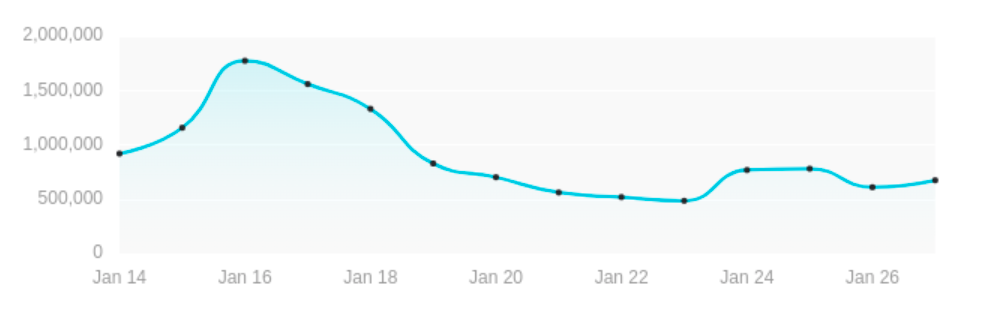
\includegraphics[scale=0.5]{fig/count_of_tr.png}
    \caption{Количество транзакций обработанных в NEAR за последние 14 дней. Дата: 28.01.2022. \url{https://explorer.near.org}} \label{fig:count_of_tr}
\end{figure}

Самая важная концепция NFT - это то, что он дает право доказать, что данный конкретный файл, интеллектуальная собственность, часть данных принадлежит конкретному одному человеку. Если в современном мире права на картину, музыку либо любой другой медиа объект хранятся на каком-нибудь сервере и подкрепляются бумажной подписью на каком-нибудь документе и не без помощи юристов, то NFT позволяет упростить весь этот процесс ненужной бумажной волокиты. Немногие готовы перенести права картины на NFT, но на сегодняшний день есть и примеры, например, блокчейн-компания <<Injective Protocol>> купила картину <<Morons>> художника Бэнкси и сожгла ее в прямом эфире, чтобы в последствии перевести данную картину в NFT\footnote{https://rg.ru/2021/03/04/zachem-sozhgli-kartinu-benksi-za-95-tysiach-dollarov.html}.

Наш маркетплейс строиться на довольно новом блокчейне и будет использоваться непременно как бот, чего я еще не видел. Наверное, такого нет в качестве бота, из-за того, что многие думают, что невозможно предоставить хороший интерфейс для этого, но это совсем неверное представление, ведь Discord API предоставляет невероятный функционал, чтобы пользователю было удобно. Также я не еще не видел такого маркетплейса, где есть хоть какая-нибудь технология связанная с машинным обучением: рекомендация цены за NFT, рекомендации самих NFT, GAN NFT картинок.
